\documentclass[tikz,border=8pt]{standalone}
\usepackage{amsmath}
\usetikzlibrary{arrows.meta,positioning,fit}

\begin{document}
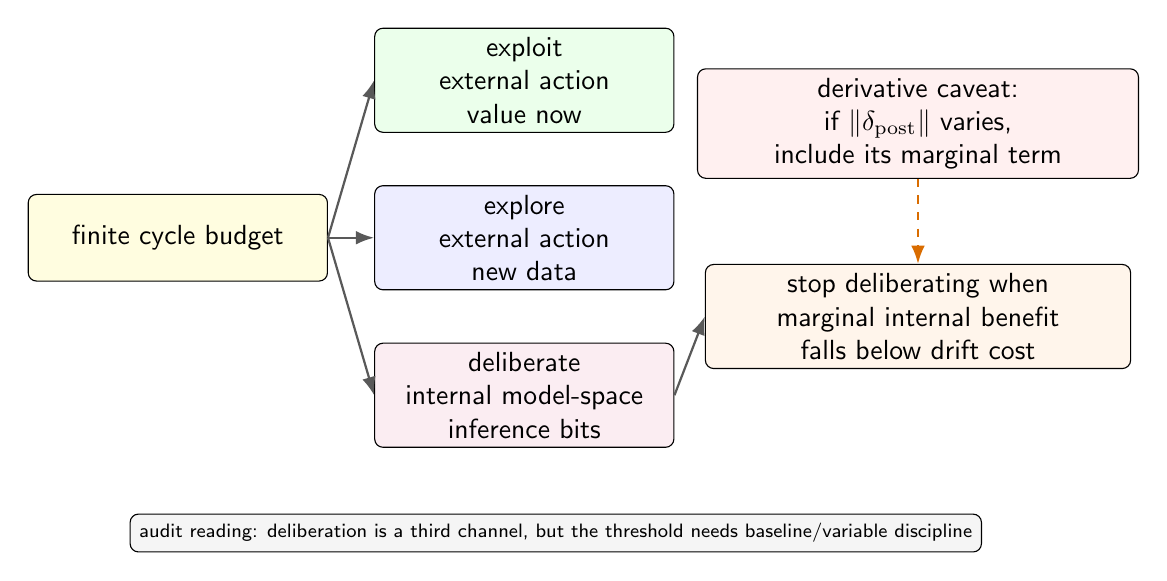
\begin{tikzpicture}[
  font=\sffamily,
  box/.style={draw, rounded corners=3pt, align=center, minimum width=38mm, minimum height=11mm, fill=white},
  note/.style={align=center, font=\sffamily\scriptsize},
  arrow/.style={-Latex, thick, draw=black!65},
  warn/.style={-Latex, thick, dashed, draw=orange!85!black}
]

\node[box, fill=yellow!12] (budget) at (0,0)
  {finite cycle budget};
\node[box, fill=green!8] (exploit) at (4.4,2)
  {exploit\\external action\\value now};
\node[box, fill=blue!7] (explore) at (4.4,0)
  {explore\\external action\\new data};
\node[box, fill=purple!7] (delib) at (4.4,-2)
  {deliberate\\internal model-space\\inference bits};

\draw[arrow] (budget.east) -- (exploit.west);
\draw[arrow] (budget.east) -- (explore.west);
\draw[arrow] (budget.east) -- (delib.west);

\node[box, fill=orange!8, minimum width=54mm] (stop) at (9.4,-1)
  {stop deliberating when\\marginal internal benefit\\falls below drift cost};
\draw[arrow] (delib.east) -- (stop.west);

\node[box, fill=red!6, minimum width=56mm] (deriv) at (9.4,1.45)
  {derivative caveat:\\if $\lVert\delta_{\rm post}\rVert$ varies,\\include its marginal term};
\draw[warn] (deriv.south) -- (stop.north);

\node[note, fill=gray!8, draw, rounded corners=3pt, minimum width=88mm] at (4.8,-3.75)
  {audit reading: deliberation is a third channel, but the threshold needs baseline/variable discipline};

\end{tikzpicture}
\end{document}
